\model{Vigen\`{e}re Cipher}

Vigen\`{e}re Ciphers are a value-added Caesar Cipher that is very difficult to crack.
Instead of using a single number, the key is a word.
Each character in the key is encoded with its own Caesar Cipher.
For example, here is how you encrypt the word \texttt{UMBRELLA} using the key \texttt{DOG} shown below.

\begin{table}[h]
\centering
\begin{tabular}{lll}
1. & Enter plaintext: & \texttt{UMBRELLA} \\[1ex]
2. & Apply the key:   & \texttt{DOGDOGDO} \\[1ex]
3. & Get ciphertext:  & \texttt{XAHUSROO}
\end{tabular}
\end{table}

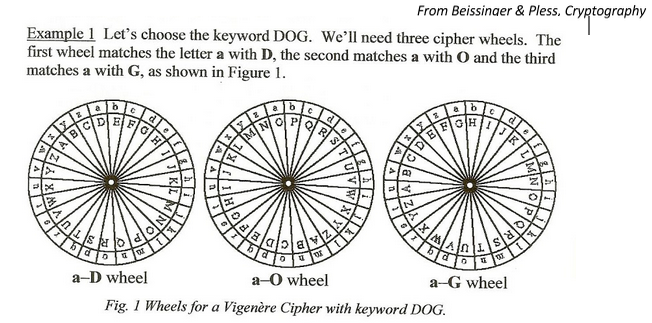
\includegraphics[width=\linewidth]{CSP/vigenere1.png}


\quest{20 min}

\Q Which letters in \texttt{UMBRELLA} use:

\begin{enumerate}
\setlength\itemsep{1em}

\item the a-D wheel for encryption? \ans{U, R, L}

\item the a-O wheel for encryption? \ans{M, E, A}

\item the a-G wheel for encryption? \ans{B, L}

\end{enumerate}
\vspace{1em}


\Q Why do you think the online cipher wheel uses lower-case letters for the outer wheel and upper-case letters for the inner wheel?

\begin{answer}
To make it easier to see the difference between plaintext and ciphertext.
\end{answer}


\Q If you were encrypting the word \texttt{PEANUT} using the keyword \texttt{CAT}, list which letters would use which cipher wheel.

\begin{answer}
\centering
C: P, N
\hspace{3em}
A: E, U
\hspace{3em}
T: A, T
\end{answer}


\Q Encrypt \texttt{PEANUT} using the keyword \texttt{CAT}.

\begin{answer}
\texttt{RETPUM} ~ (the first key is 2, the second is 0, the third is 19)
\end{answer}


\Q Consider the length of the keyword.

\begin{enumerate}
\setlength\itemsep{1em}

\item If we knew the keyword was two letters long, how many combinations of cipher wheels are there? Show your work.

\ans{26 * 26 = 676}

\item If we knew the keyword was three letters long, how many combinations of cipher wheels are there? Show your work.

\ans{26 * 26 * 26 = 17,576}

\item Ideally, if we needed to encrypt a 1000 character document, how long should the keyword be? Explain your answer.

\begin{answer}
The longer the keyword, the more secure it is.
However, at some point it's not worth the extra computation.
Plus there's only 26 unique letters. 12-15 is practically enough.
\end{answer}

\end{enumerate}


\Q Think about the examples you brainstormed at the beginning of the activity.
What is one advantage and one disadvantage of using Vigen\`{e}re Cipher encryption for online security?

\begin{enumerate}
\setlength\itemsep{1em}

\item one advantage:

\ans{It's still relatively simple to compute, and more secure than Caesar ciphers.}

\item one disadvantage:

\ans{The key is more complex, and it may be slower to perform the encryption.}

\end{enumerate}
